\documentclass[tikz, border=8pt]{standalone}
\usepackage{amsmath,amssymb,bm}
\usetikzlibrary{arrows.meta, positioning, calc}

% ── Node styles ─────────────────────────────────────────────────────────────
\tikzset{
  base/.style={
    draw, rounded corners=3pt,
    minimum width=4.2cm, minimum height=0.85cm,
    text width=4.0cm, align=center,
    font=\small,
  },
  envbox/.style ={base, fill=blue!7,    draw=blue!45!black,  line width=0.6pt},
  obsbox/.style ={base, fill=orange!8,  draw=orange!60!black,line width=0.6pt},
  pfbox/.style  ={base, fill=violet!8,  draw=violet!55!black,line width=0.6pt},
  polbox/.style ={base, fill=green!7,   draw=green!55!black, line width=0.6pt},
  arr/.style    ={-{Stealth[length=4.5pt,width=3pt]}, line width=0.7pt, black!70},
  arrlbl/.style ={midway, right=1pt, font=\scriptsize, text=black!60,
                  fill=white, inner sep=1pt},
}

\begin{document}
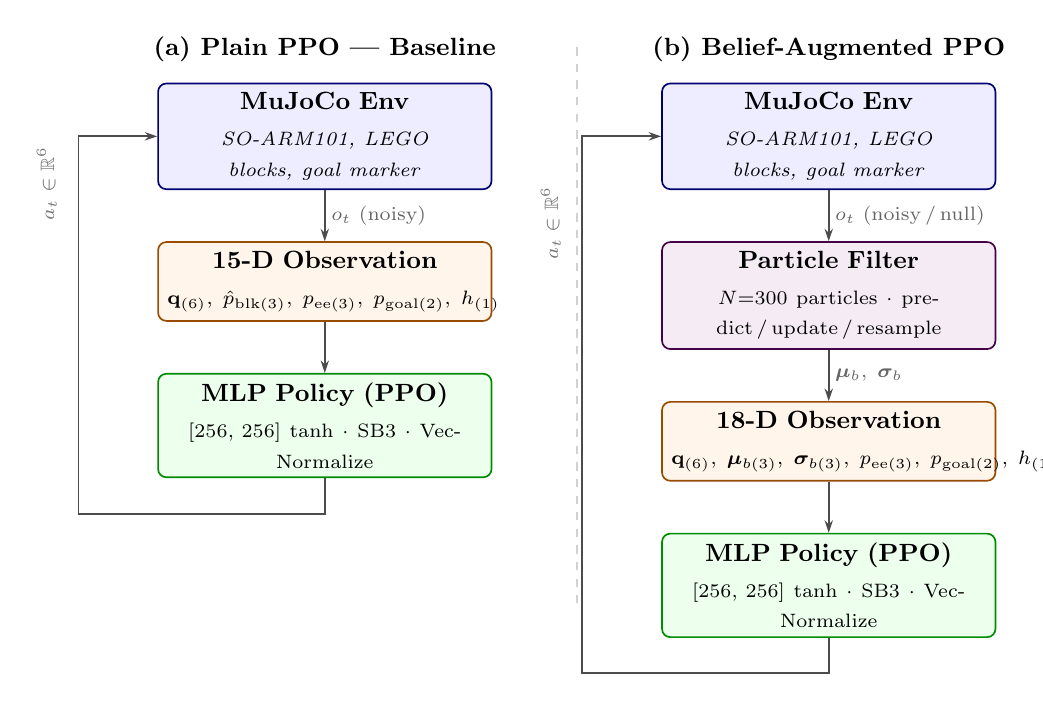
\begin{tikzpicture}[node distance=6.5mm]

%% ════════════════════════════════════════════════════════════
%%  LEFT PANEL — Plain PPO
%% ════════════════════════════════════════════════════════════
\node[envbox] (pe)
  {\textbf{MuJoCo Env}\\[2pt]
   \scriptsize\textit{SO-ARM101, LEGO blocks, goal marker}};

\node[obsbox, below=of pe] (po)
  {\textbf{15-D Observation}\\[2pt]
   \scriptsize
   $\mathbf{q}_{(6)},\;
    \hat{p}_{\text{blk}(3)},\;
    p_{\text{ee}(3)},\;
    p_{\text{goal}(2)},\;
    h_{(1)}$};

\node[polbox, below=of po] (pp)
  {\textbf{MLP Policy (PPO)}\\[2pt]
   \scriptsize $[256,\,256]$~tanh~$\cdot$~SB3~$\cdot$~VecNormalize};

% arrows down
\draw[arr] (pe.south) -- (po.north)
  node[arrlbl] {$o_t$~(noisy)};
\draw[arr] (po.south) -- (pp.north);

% action feedback loop — left side
\coordinate (pfbl) at ($(pp.south west) + (-1.0cm, 0)$);
\coordinate (pebl) at ($(pe.north west) + (-1.0cm, 0)$);
\draw[arr]
  (pp.south) -- ++(0,-0.45cm) -|
  ($(pp.west) + (-1.0cm, -0.2cm)$) --
  ($(pe.west)  + (-1.0cm,  0.0cm)$) --
  (pe.west);
\node[font=\scriptsize, text=black!55, rotate=90, anchor=south]
  at ($(pe.west) + (-1.15cm, -0.6cm)$) {$a_t\in\mathbb{R}^6$};

% panel title
\node[font=\small\bfseries, above=4pt of pe]
  {(a)~Plain PPO — Baseline};

%% ════════════════════════════════════════════════════════════
%%  RIGHT PANEL — Belief-Augmented PPO
%% ════════════════════════════════════════════════════════════
\begin{scope}[xshift=6.4cm]

\node[envbox] (be)
  {\textbf{MuJoCo Env}\\[2pt]
   \scriptsize\textit{SO-ARM101, LEGO blocks, goal marker}};

\node[pfbox, below=of be] (bf)
  {\textbf{Particle Filter}\\[2pt]
   \scriptsize
   $N{=}300$~particles~$\cdot$~predict\,/\,update\,/\,resample};

\node[obsbox, below=of bf] (bo)
  {\textbf{18-D Observation}\\[2pt]
   \scriptsize
   $\mathbf{q}_{(6)},\;
    \bm{\mu}_{b(3)},\;
    \bm{\sigma}_{b(3)},\;
    p_{\text{ee}(3)},\;
    p_{\text{goal}(2)},\;
    h_{(1)}$};

\node[polbox, below=of bo] (bp)
  {\textbf{MLP Policy (PPO)}\\[2pt]
   \scriptsize $[256,\,256]$~tanh~$\cdot$~SB3~$\cdot$~VecNormalize};

% arrows down
\draw[arr] (be.south) -- (bf.north)
  node[arrlbl] {$o_t$~(noisy\,/\,null)};
\draw[arr] (bf.south) -- (bo.north)
  node[arrlbl] {$\bm{\mu}_b,\;\bm{\sigma}_b$};
\draw[arr] (bo.south) -- (bp.north);

% action feedback loop — left side
\draw[arr]
  (bp.south) -- ++(0,-0.45cm) -|
  ($(bp.west) + (-1.0cm, -0.2cm)$) --
  ($(be.west) + (-1.0cm,  0.0cm)$) --
  (be.west);
\node[font=\scriptsize, text=black!55, rotate=90, anchor=south]
  at ($(be.west) + (-1.15cm, -1.1cm)$) {$a_t\in\mathbb{R}^6$};

% panel title
\node[font=\small\bfseries, above=4pt of be]
  {(b)~Belief-Augmented PPO};

\end{scope}

%% vertical separator
\draw[black!18, line width=0.6pt, dashed]
  ($(pe.north east)!0.5!(be.north west) + (0, 0.45cm)$)
  --
  ($(pp.south east)!0.5!(bp.south west) + (0,-0.6cm)$);

\end{tikzpicture}
\end{document}
